
\section{5.对易关系的物理含义}

\begin{frame}
    \frametitle{前情回顾}
    \begin{itemize}
        \Item 希尔伯特空间的态矢量描述体系状态
        \Item 希尔伯特空间的算符给出体系的物理量
        \Item 算符的本征函数系构成正交归一完全基
        \Item 常见算符本征方程求解
        \Item 算符对易关系
    \end{itemize}   
\end{frame} 

\subsection{对易的物理含义}

\begin{frame} 
    \frametitle{对易的含义}
    \begin{enumerate}
        \Item  相互对易的两力学量算符,具有共同本征函数系
        \Item  当体系处于共同的本征态时,它们同时具有确定值
        \Item  构成最小完全集的一组力学量算符的数目等于体系的自由度。
    \end{enumerate}
\end{frame} 

\begin{frame} [allowframebreaks=]
    \begin{tcolorbox1}{定理1:}
        如果两算符具有共同的本征函数系,则它们对易
    \end{tcolorbox1}
    \alert{证明:} 设它们的共同本征函数系为{$\varphi_n$}, 有:\\ 
        \begin{equation*}
            \begin{split} 
            A\varphi_n&=a_n \varphi_n \\
            B\varphi_n&=b_n \varphi_n \\
            \end{split}  
        \end{equation*}  
        对任意波函数
        \begin{equation*}
            \begin{split} 
            [A,B]\Psi &= [A,B]\sum_n c_n \varphi_n \\
            &= \sum_n c_n [A,B]\varphi_n \\
            &= \sum_n c_n (AB-BA)\varphi_n\\
            &= \sum_n c_n AB\varphi_n- \sum_n c_n BA\varphi_n\\
            &= \sum_n c_n a_nb_n\varphi_n- \sum_n c_n a_nb_n\varphi_n\\
            &=0\Psi
            \end{split}  
        \end{equation*}  
        得证: $$[A,B]=0$$
\end{frame} 

\begin{frame} [allowframebreaks=]
    \begin{tcolorbox1}{逆定理:}
       如果两算符对易,则它们具有共同的本征函数系。
    \end{tcolorbox1}
    \alert{证明:} 设A有本征函数系{$\varphi_n$}, 有:\\ 
        \begin{equation*}
            \begin{split} 
            A(B\varphi_n)&= AB\varphi_n\\
            &=BA\varphi_n \\
            &=Ba_n\varphi_n \\
            &=a_n(B\varphi_n) \\
            \end{split}  
        \end{equation*}  
        说明$B\varphi_n$ 和 $\varphi_n$ 都是A的属于本征值$a_n$的本征态,当$a_n$非简并时, 
        $B\varphi_n$ 和 $\varphi_n$ 描述同一个态,两者最多只差一个常数因子,记为 $b_n$,
        $$ B\varphi_n=b_n \varphi_n$$
        即: $\varphi_n$也是B的本征态。\\
        证毕!
\end{frame} 

\begin{frame} [allowframebreaks=]
    \begin{tcolorbox1}{推论1:}
        一组力学量算符具有共同本征函数完备系的充要条件是这些算符彼此两两对易
    \end{tcolorbox1}
    \alert{例子1:动量本征函数系} \\
    由于 $[p_\alpha,p_\beta]=0$,动量算符($p_x, p_y, p_z$)具有共同本征函数系 即平面波\\
    $$ \Psi_{\vec p}= \frac{1}{(2\pi\hbar)^{3/2}} e^{\frac{i}{\hbar}\vec{p}\cdot\vec{r}}$$ 
    \alert{例子2:角动量本征函数系} \\
    由于 $[L_z,L^2]=0$,它们具有共同的本征函数系 {$Y_{lm}$},\\
    当体系处于共同的本征态$Y_{lm}$时 ,它们同时具有确定值
    $$L_z= m\hbar, \qquad L^2=l(l+1)\hbar ^2 $$.
    当体系处于非共同的本征态,比如 $\frac{1}{\sqrt{2}}Y_{lm} + \frac{1}{\sqrt{2}}Y_{lm'}$,此时,$L^2$具有确定值
    $$L^2=l(l+1)\hbar ^2 $$,
    而$L_z$具有两个可能值(非确定)
    $$L_z= m\hbar\quad \text{or} \quad m'\hbar$$
    也就是说$\frac{1}{\sqrt{2}}Y_{lm} + \frac{1}{\sqrt{2}}Y_{lm'}$依然是$L^2$的本征态,却不是$L_z$的本征态。
\end{frame} 

\begin{frame}
    \begin{tcolorbox1}{推论2:}
        一组力学量同时有确定值的条件:一组力学量算符具有共同本征函数完备系的充要条件是这些算符彼此两两对易
    \begin{enumerate}
    \Item 算符彼此两两对易
    \Item 体系处于共同本征态
    \end{enumerate}
    \end{tcolorbox1}

\end{frame} 

\begin{frame} [allowframebreaks=]
    \begin{tcolorbox1}{推论3:}
        完全确定体系的一个量子态所需要的彼此对易的一组力学量算符集称为力学量完全集,最小力学量完全集所含力学量的数目等于体系的自由度。
    \end{tcolorbox1}
    \alert{例子1:空间的自由度为3} \\
    完全确定空间一个矢量(一个点)的位置,至少需要三个彼此对易的一组力学量构成的集,比如: $$(i,j,k) \qquad or \qquad (r,\theta,\varphi) $$
    当然,你可以用多于三个力学量构成的集来完全描述,但不是最小完全集!\\
\end{frame} 

\begin{frame}
    \alert{例子2:经典物理学} \\
    经典物理学用$\vec{r}, \vec{p}$来完全描述质点的运动状态,用了六个力学量$(x,y,z, p_x, p_y, p_z)$,量子力学发现这个集并不是彼此对易的,
    $$\begin{cases}
        [x_\alpha,x_\beta]= 0  \\ 
        [p_\alpha,p_\beta]= 0  \\ 
        [x_\alpha,p_\beta]= i\hbar \delta_{\alpha\beta}  \\ 
    \end{cases}$$
    它们不能构成一个完全集!
\end{frame} 

\subsection{不对易的物理含义}

\begin{frame} 
    \frametitle{不对易的含义}
    \begin{tcolorbox1}{不确定性原理:}
        两不对易力学量算符,一般不同时具有确定值    
    \end{tcolorbox1}
\end{frame} 

\begin{frame} 
    \frametitle{不确定度}
    \begin{itemize}
        \Item 偏差: 测量值与平均值之差
        $$ \Delta F=F-\bar{F} $$
        \Item 不确定度: 偏差的绝对值
         $$ \left | \Delta F  \right | $$
        \Item 均方差: 偏差平方的平均值 (量子涨落)
        $$ \overline{(\Delta F)^2} = \overline{F^2} - \overline{F}^2$$
    \end{itemize}   
    我们通常先算(1)算符的平方的平均值和(2)算符的平均值平方,得到了均方差,再开方得到不确定度!
\end{frame} 

\begin{frame} 
    \frametitle{}
    \alert{证明:}
    \begin{equation*}
        \begin{split} 
        \overline{(\Delta F)^2}&= \overline{(F-\bar{F})^2}\\
        &=\overline{F^2-2F\bar{F}+\bar{F}^2 }\\
        &=\overline{F^2} -2\overline{F\bar{F}} +\overline{\bar{F}^2 }\\
        &=\overline{F^2} -2\overline{F}^2 +\overline{F}^2\\
        &= \overline{F^2} - \overline{F}^2
        \end{split}  
    \end{equation*} 
\end{frame} 

\begin{frame} 
    \frametitle{}
    \begin{tcolorbox2}{不确定度对易关系}
     试证明:  $$[\Delta F, \Delta G]= [F, G]$$
    \end{tcolorbox2}
    \alert{证明:}
    \begin{equation*}
        \begin{split} 
        [\Delta F, \Delta G]&= \Delta F \Delta G - \Delta G \Delta F \\
        &=(F-\bar{F}) (G-\bar{G})- (G-\bar{G}) (F-\bar{F}) \\
        &=FG -F\bar{G}-\bar{F}G + \bar{F} \bar{G} -GF + G \bar{F} + \bar{G} F -\bar{G} \bar{F}   \\
        &=FG-GF \\
        &=[F, G]
        \end{split}  
    \end{equation*} 
\end{frame} 

\begin{frame} [allowframebreaks=]
    \frametitle{}
    \alert{不确定性原理的严格证明:} \\
    令 $[\hat{F}, \hat{G}]= i\hat{k}$,对任意波函数,计算含实参$\xi$的积分:
    $$
    \begin{aligned}
    I(\xi)= &\int|(\xi\Delta \hat{F}-i \Delta \hat{G}) \psi|^{2} d \tau \quad (\geq 0) \\
    =&\int[\xi \Delta \hat{F} \psi-i \Delta \hat{G} \psi][\xi \Delta \hat{F} \psi-i \Delta \hat{G} \psi]^{*} d \tau \\
    =&\int[\xi \Delta \hat{F} \psi-i \Delta \hat{G} \psi] [\xi(\Delta \hat{F} \psi)^{*}+i(\Delta \hat{G} \psi)^{*}] d \tau \\
    =&\int[\xi \Delta \hat{F} \psi-i \Delta \hat{G} \psi]\left[\xi(\Delta \hat{F} \psi)^{*}+i(\Delta \hat{G} \psi)^{*}\right] d \tau \\
    =& \xi^{2} \int(\Delta \hat{F} \psi)(\Delta \hat{F} \psi) * d \tau-i \xi \int(\Delta \hat{G} \psi)(\Delta \hat{F} \psi) * d \tau \\
        &+i \xi \int(\Delta \hat{F} \psi)(\Delta \hat{G} \psi) * d \tau+\int(\Delta \hat{G} \psi)(\Delta \hat{G} \psi) * d \tau \\
    \end{aligned}
    $$
    $$
    \begin{aligned}
    =& \xi^{2} \int \psi^{*}(\Delta \hat{F})^{2} \psi d \tau-i \xi \int \psi^{*}(\Delta \hat{F} \Delta \hat{G}) \psi d \tau \\
    &+i \xi \int \psi^{*}(\Delta \hat{G} \Delta \hat{F}) \psi d \tau+\int \psi^{*}(\Delta \hat{G})^{2} \psi d \tau \\
    =& \xi^{2} \int \psi^{*}(\Delta \hat{F})^{2} \psi d \tau-i \xi \int \psi^{*}(\Delta \hat{F} \Delta \hat{G}-\Delta \hat{G} \Delta \hat{F}) \psi d \tau+\int \psi^{*}(\Delta \hat{G})^{2} \psi d \tau \\
    =& \xi^{2} \overline{(\Delta F)^{2}}-i \xi \overline{[\Delta F, \Delta G]}+\overline{(\Delta G)^{2}}\\
    =&\xi^{2} \overline{(\Delta F)^{2}}+\xi \overline{[F, G]}+\overline{(\Delta G)^{2}} \\
    =&\xi^{2} \overline{(\Delta F)^{2}}+\xi \bar{\hat{k}}+\overline{(\Delta G)^{2}} \\
    \geq & 0\\
    \end{aligned}
    $$
\end{frame} 

\begin{frame} 
    \[\xi^{2} \overline{(\Delta F)^{2}}+\xi \bar{\hat{k}}+\overline{(\Delta G)^{2}} \geq  0\]  
    对比不等式条件:
    $$
    a \xi^{2}+b \xi+c \geq 0
    $$
    $$
    b^{2}-4 a c \leq 0 \Rightarrow a c \geq \frac{b^{2}}{4}
    $$
    可知: 
    $$
    \overline{(\Delta \hat{F})^{2}} \cdot \overline{(\Delta \hat{G})^{2}} \geq \frac{(\bar{\hat{k}})^{2}}{4}
    $$
    得: 
    $$
    \overline{(\Delta \hat{F})^{2}} \cdot \overline{(\Delta \hat{G})^{2}} \geq \frac{1}{4}|\overline{[\hat{F}, \hat{G}]}|^{2}
    $$
    证毕!
\end{frame} 

\begin{frame}
取位置与动量为例,有:
$$ [x,p_x]=i\hbar $$
$$
\overline{(\Delta \hat{x})^{2}} \cdot \overline{(\Delta \hat{p_x})^{2}} 
\geq \frac{1}{4}|\overline{[\hat{x}, \hat{p_x}]}|^{2}=\frac{\hbar^2}{4}
$$
$$
\sqrt{\overline{(\Delta x)^{2}} \cdot \overline{(\Delta p_x)^{2}}} 
\geq \frac{\hbar}{2}
$$
$$  
\Delta x \cdot \Delta p_x 
\geq \frac{\hbar}{2}
$$ 
得位置-动量不确定性关系,称为海森堡不确定性关系.
\end{frame}

\begin{frame}
    能量-时间不确定性关系:
    \[\Delta x \Delta p = \Delta (vt)  \Delta p = \Delta t  \Delta (vp_x)= \Delta t  \Delta E \]
    \[\to \Delta E \Delta t \geq \frac{\hbar}{2}  \]
    激发态没有明确的能量,其能量不确定度$\Delta E$也称为能级宽度$\Gamma$,\\
    根据不确定性有理,$\Gamma$越大(越扩展),粒子处于这个态的寿命越短;$\Gamma$越小(越局域),
    粒子处于这个态的寿命越长。\\
    在光谱中体现为:峰宽(1/2峰高处的展宽)越大,对应的态寿命越短;峰宽越小,态越稳定。 
\end{frame}

\begin{frame}
    \frametitle{海森堡}
    \begin{wrapfigure} {r} {0.3\textwidth} %;图在右
        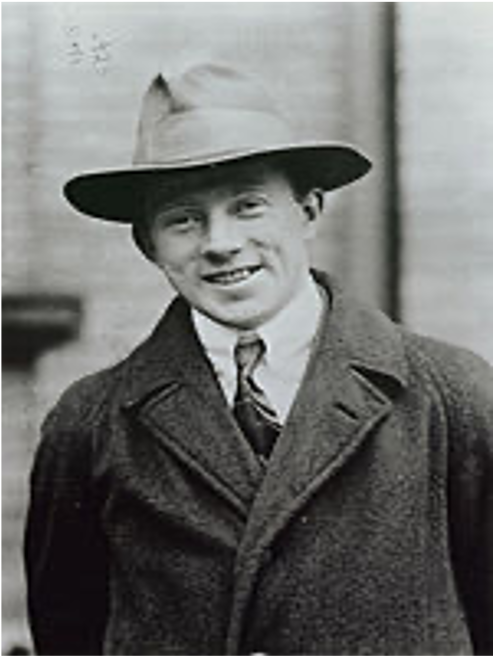
\includegraphics[width=0.25\textwidth]{figs/hesb.png}   
    \end{wrapfigure}
    维尔纳·海森堡(Werner Heisenberg,1901年12月5日-1976年2月1日),德国物理学家,1932年诺贝尔物理学奖。主要贡献:(1) 创立矩阵力学(量子力学的矩阵形式);(2)提出“测不准原理”;(3)散射(S)矩阵。  
\end{frame}

\begin{frame} [allowframebreaks=]
    \begin{tcolorbox2}{不确定性关系式表明:}
    \begin{itemize}
        \Item 若两个力学量算符不对易(对易子不等于零),对易子平均值的平方一般大于零,则它们的不确定度的积必大于零,说明它们一般不能同时具有确定值
        \Item 若两个力学量算符对易,则总可以找出这样的态(比如共同的本征态),使它们同时有确定值。 
    \end{itemize}   
    \end{tcolorbox2}
\end{frame} 

\begin{frame} [allowframebreaks=]
    TIPS:下列说法,正确的有:
    \begin{enumerate}
        \Item 两力学量算符对易,则同时有确定值。 
        \Item 两力学量算符不对易,则不能同时有确定值 
        \Item 若两力学量算符有共同的本征态,则彼此对易
        \Item 若两力学量算符不对易,则没有共同本征态
        \Item 若[A,B]=常数,则A和B能有共同本征态
    \end{enumerate} 
\end{frame} 

\begin{frame} 
    \frametitle{}
    \begin{tcolorbox2}{课堂作业}
    已知$[L_x, L_y]=i\hbar L_z$, 试计算体系处于$L_z$的基态 $$Y_{00}=\frac{1}{\sqrt{4\pi}}$$时,$L_x, L_y$的不确定度。
    \end{tcolorbox2}
\end{frame} 

\begin{frame} 
    \frametitle{}
    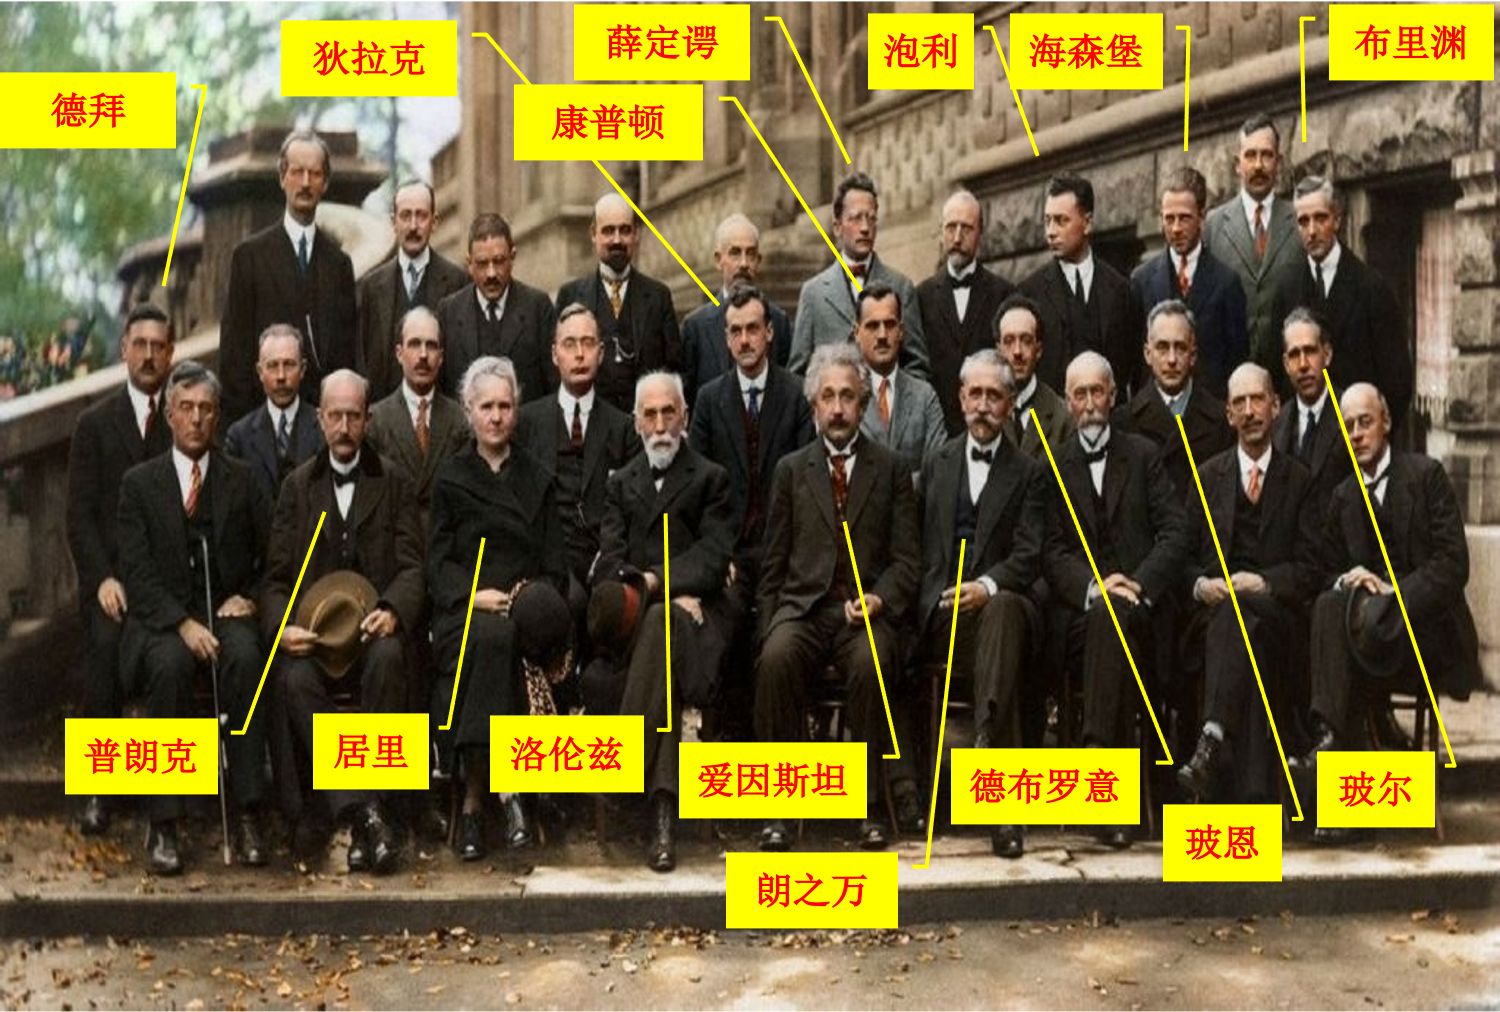
\includegraphics[width=0.9\textwidth]{figs/meet.png}
\end{frame} 

